\documentclass{sfuthesis}

\title{fill in title}
\thesistype{Master}
\author{Marten Heidemeyer}
\previousdegrees{%
	B.Sc., Universit{\"a}t zu L{\"u}beck, 2013}
\degree{Master of Science}
\discipline{Computing Science}
\department{Department of Computing Science}
\faculty{}
\copyrightyear{2016}
\semester{Fall 2016}
\date{1 September 2015}

\keywords{}

\committee{%
	\chair{}{}
	\member{}{Senior Supervisor\\Professor}
	\member{}{Supervisor\\Associate Professor}
	\member{}{Supervisor\\Adjunct Professor}
	\member{}{Internal Examiner\\Assistant Professor\\School of Engineering Science}
	\member{}{External Examiner\\Professor\\Department of Quantum Fields\\Mars University}
}

%   PACKAGES AND CUSTOMIZATIONS  %%%%%%%%%%%%%%%%%%%%%%%%%%%%%%%%%%%%%%%%%%%%%%
%
%   Add any packages or custom commands you need for your thesis here.
%   You don't need to call the following packages, which are already called in
%   the sfuthesis class file:
%
%   - appendix
%   - etoolbox
%   - fontenc
%   - geometry
%   - lmodern
%   - nowidow
%   - setspace
%   - tocloft
%
%   If you call one of the above packages (or one of their dependencies) with
%   options, you may get a "Option clash" LaTeX error. If you get this error,
%   you can fix it by removing your copy of \usepackage and passing the options
%   you need by adding
%
%       \PassOptionsToPackage{<options>}{<package>}
%
%   before \documentclass{sfuthesis}.
%

\usepackage{amsmath,amssymb,amsthm}
\usepackage[pdfborder={0 0 0}]{hyperref}
\usepackage{graphicx}
\usepackage{caption}
\usepackage{tikz}
\usepackage{mathrsfs}

\DeclareMathOperator*{\argmax}{argmax}






%   FRONTMATTER  %%%%%%%%%%%%%%%%%%%%%%%%%%%%%%%%%%%%%%%%%%%%%%%%%%%%%%%%%%%%%%
%
%   Title page, committee page, copyright declaration, abstract,
%   dedication, acknowledgements, table of contents, etc.
%

\begin{document}

\frontmatter
\maketitle{}
%\makecommittee{}

\begin{abstract}
	
\end{abstract}

\begin{dedication} % optional
\end{dedication}

\begin{acknowledgements} % optional
\end{acknowledgements}

\addtoToC{Table of Contents}\tableofcontents\clearpage
\addtoToC{List of Tables}\listoftables\clearpage
\addtoToC{List of Figures}\listoffigures

%   MAIN MATTER  %%%%%%%%%%%%%%%%%%%%%%%%%%%%%%%%%%%%%%%%%%%%%%%%%%%%%%%%%%%%%%
%
%   Start writing your thesis --- or start \include ing chapters --- here.
%

\mainmatter%


\chapter{Introduction}

\section{A Statement of the Problem}

Knowledge about the interaction strength between chemical structures and proteins is an important topic in drug development.
The goal in drug development is to find a chemical structure that binds to a diseases target protein without causing harmful side effects by binding to proteins other than the diseases target.
The safest and most accurate method to gain knowledge about the interaction strength of drug candidates and target proteins is through wetlab experiments. On the other hand, wetlab experiments are costly in terms of time and money, as there are thousands of potential drug candidates. The failure of a new ligand in toxicity tests is higher than $90\%$ which is the most significant reason for the high cost of the drug development process. In drug development, drug repositioning is a technique in which known drugs and drug candidates are used to treat new diseases. Existing drugs may bind to the target protein of a disease other than the disease that the drug was originally developed for. Using an existing drug as a basis for the development of a new drug is far more likely to succeed, because the existing drug has already passed toxicity tests and its safety is known. Numerous openly accessible databases exist, listing the interaction of known compounds, which can be either already approved drugs or experimental drug candidates, against known target proteins (ChEMBL \cite{gaulton2012chembl}, DrugBank \cite{wishart2008drugbank}, KEGG\cite{kanehisa2011kegg}, SuperTarget \cite{gunther2008supertarget}, BindingDB \cite{liu2007bindingdb}). 

\section{Review of Literature}

Machine Learning and Data Mining techniques for drug development is a hot topic. In most existing methods the problem is formulated as a binary classification problem, where the drug-target pairs are treated as instances and the chemical structures of drugs and the amino acid subsequences of the targets can be used as features, describing the instances. The goal in the binary formulation is to classify a given drug-target pair into binding and non binding.

Two existing methods for drug target interaction prediction that are not based on machine learning techniques are docking simulation and ligand-based approaches. In docking simulation the interaction strength of ligands and proteins is estimated based on the structure of the target protein. This process is extremely time-consuming and the structural information of a protein is not always available \cite{liu2016neighborhood}. In ligand based approaches, the interaction strength of a candidate ligand to a target protein is obtained by comparing the candiate ligand to ligands for which the interaction strength to the target is known. This approach is not applicable, when information of candidate-similar ligands is not available for the target protein.

\input{Method.tex}

\section{Datasets}

In the majority of studies that can be found in the literature, the presented models for drug target interaction prediction are trained and evaluated on binary datasets. Typically the existing models are evaluated on the four datasets that were first presented in \cite{yamanishi2010drug}. In these datasets a label of $y_{d_i, t_j} = 1$ is given for a drug-target pair $(d_i, t_j)$ which is known to interact and a label of $y_{d_i, t_j} = 0$ is given when either the drug-target pair is known not to interact or when it is unknown whether the pair interacts. In contrast to a model that classifies if a drug-target pair interacts or not, the model that is developed in this thesis predicts the continuous binding affinity of drug target pairs. To the best of my knowledge, only one existing study can be found in the literature which presents a model for the prediction of the continuous binding affinity of drugs and targets \cite{pahikkala2014toward}. This study utilizes two continuous datasets (\textit{Metz} and \textit{Davis}) that are also used in this thesis to evaluate and compare the developed model. A third dataset \textit{KIBA} is obtained by preprocessing the drug-target dataset that is presented in \cite{tang2014making}.
The three datasets named \textit{Metz}, \textit{Davis} and \textit{KIBA} respectively that are used for evaluating the developed model and for comparing it to the model presented in \cite{pahikkala2014toward} are described in the following chapters. Additionally, each section describes the corresponding drug-drug and target-target similarity matrices that were used to construct the graphical model of the CCRF.

\subsection{The Davis Dataset}

The continuous dataset \textit{Davis} was used for the evaluation of the drug-target interaction prediction model presented in \cite{pahikkala2014toward}. The dataset itself was published in the study \cite{davis2011comprehensive}. For this dataset, the interaction of 72 kinase inhibitors with 442 kinases was tested and measured as the $K_d$ value. The kinase inhibitors are the drugs and the kinases are the targets in the more general formulation of drugs and targets. The \textit{Davis} dataset contains the full information of binding affinities for all drug-target pairs in the dataset, and thus contains no missing values. The binding affinities are measured as $K_d$ values. A lower $K_d$ value represents a higher binding affinity between the drug and the target. As described in \cite{davis2011comprehensive}, the binding affinity is not reported if it was measured to be $>10000$. For these drug target pairs, a $K_d$ value of $10000$ was imputed for the experiments in this thesis.
The $K_d$ values in the \textit{Davis} dataset were log transform, according to the formula:

\begin{equation}
pK_d:= -log_{10}(\frac{K_d}{1e9})
\end{equation}

As drug-drug and target-target similarities for this dataset the matrices were used that can be downloaded from the website of the author of \cite{pahikkala2014toward}.

\begin{figure}
\begin{center}
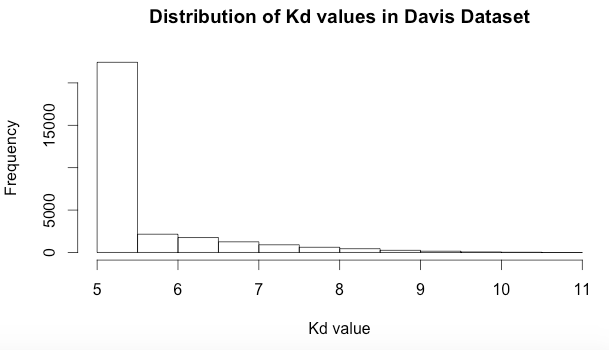
\includegraphics[scale=0.6]{davis_dist.png}
\end{center}
\caption{Distribution of $K_d$ values given in the Davis dataset.}
\label{fig:numStructure}
\end{figure}

\subsection{The Metz Dataset}

Just as the \textit{Davis} dataset, the continuous dataset \textit{Metz} was used for the evaluation of the drug-target interaction prediction model presented in \cite{pahikkala2014toward}. The dataset was published in the study \cite{metz2011navigating}. The \textit{Metz} dataset consists of 1421 drugs and 156 targets. The binding affinity is given as log transformed $K_i$ values for 42$\%$ of the drug-target pairs. As drug-drug and target-target similarities for this dataset the matrices were used that can be downloaded from the website of the author of \cite{pahikkala2014toward}.
\begin{figure}
\begin{center}
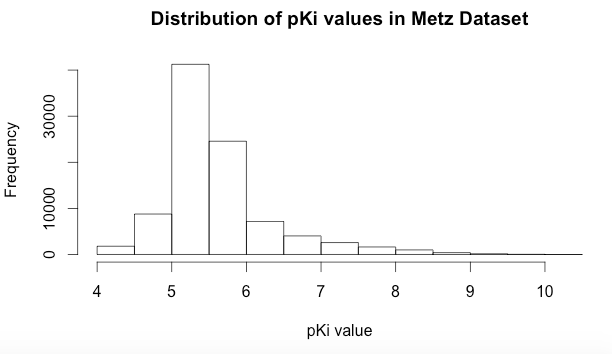
\includegraphics[scale=0.6]{metz_dist.png}
\end{center}
\caption{Distribution of $K_i$ values given in the Metz dataset.}
\label{fig:numStructure}
\end{figure}

\subsection{The KIBA Dataset}

The \textit{Davis} and \textit{Metz} datasets are suitable for the evaluation of predictive models for drug target interaction because data heterogeneity is not an issue. We can assume that the experimental settings for the measured drug target pairs in each dataset were the same and the binding affinities are comparable. When working with experimental results that come from multiple sources the data might be heterogeneous: In one case the binding affinity might be measured by $K_i$, in another case by $K_d$ and in a third case by $IC_{50}$ value. Another source of data heterogeneity are different experimental settings. An approach to integrate the observations from different sources, named \textit{KIBA} and a corresponding dataset is presented in \cite{tang2014making}. With their method, the authors of \cite{tang2014making} integrated the experimental results from multiple databases into a bioactivity matrix of 52498 compounds and 467 targets, including 246088 observations. The binding affinities in this matrix are given as \textit{KIBA}-scores. This dataset was used to obtain a third evaluation dataset, which is called the \textit{KIBA} dataset, by removing all drugs and targets with less than 10 observations from the original dataset that was downloaded from the supplementary material of \cite{tang2014making}, resulting in a dataset of 2116 drugs and 229 targets with a density of $~24\%$. For this dataset the drug-drug similarity matrix was computed through the PubChem structure clustering tool (https://pubchem.ncbi.nlm.nih.gov/assay/assay.cgi?p=clustering). The target target similarity matrix was computed by computing the normalized Smith Waterman Score \cite{yamanishi2010drug} for each pair of targets.

\begin{figure}
\begin{center}
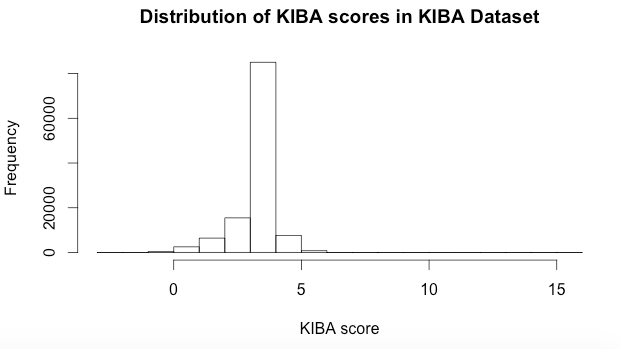
\includegraphics[scale=0.6]{kiba_dist.png}
\end{center}
\caption{Distribution of KIBA scores given in the KIBA dataset.}
\label{fig:numStructure}
\end{figure}





%   BACK MATTER  %%%%%%%%%%%%%%%%%%%%%%%%%%%%%%%%%%%%%%%%%%%%%%%%%%%%%%%%%%%%%%
%
%   References and appendices. Appendices come after the bibliography and
%   should be in the order that they are referred to in the text.
%
%   If you include figures, etc. in an appendix, be sure to use
%
%       \caption[]{...}
%
%   to make sure they are not listed in the List of Figures.
%

\backmatter%
	\addtoToC{Bibliography}
	\bibliographystyle{plain}
	\bibliography{references}

\begin{appendices} % optional
	\chapter{Code}
\end{appendices}
\end{document}
